
% !TeX spellcheck = de_DE
\documentclass[ngerman]{scrartcl} 

%\KOMAoptions{fontsize=12pt, paper=a4}
%\KOMAoptions{DIV=11}
\usepackage{float}
\usepackage[utf8]{inputenc}             % Direkte Eingabe von ä usw.
\usepackage[T1]{fontenc}               	% Font Kodierung für die Ausgabe
%\usepackage[ngerman]{babel}                   	% Verschiedenste sprach-spezifische Extras
\usepackage{parskip}
% \usepackage[autostyle=true]{csquotes}	% Intelligente Anführungszeichen
%\usepackage{amsmath}
\usepackage{amsmath,amsthm,amssymb}% Mathematischer Formelsatz mit zusätzlichen mathematischen Schriften und Symbolen
\usepackage{amssymb}					% Mathematischer Formelsatz mit zusätzlichen mathematischen Schriften und Symbolen
\usepackage{physics}					% Differentialgleichungen
\usepackage{listings}					% Zum Einbinden von Programmcode verwenden wir das listings-Paket
\usepackage[dvipsnames]{xcolor}			% um Elemente von Befehlen farblich zu unterstützen
%\usepackage[varg]{txfonts}              % Schönere Schriftart
\usepackage{graphicx}					% Paket um externe Graphiken einzufügen
\usepackage{multirow}
\usepackage{pdflscape}
\usepackage{geometry}
\usepackage{media9}
\RequirePackage[backend=biber, style=numeric]{biblatex} % Literaturverzeichnis
\usepackage{hyperref} 					% um klickbare Elemente in Ihrem PDF-Ausgabedokument zu erzeugen
\RequirePackage[all]{hypcap} 			% ergänzend zu hyperref
\usepackage[separate-uncertainty=true]{siunitx}          
\usepackage{nicefrac}
\usepackage{bbold}

% Intelligentes Setzten von Zahlen und Einheiten
\sisetup{locale = DE}
\usepackage{enumitem}					% Aufzählungsarten
\usepackage{fancyhdr}
\usepackage{verbatim}
\usepackage{ytableau}%young diagrams
\usepackage{dsfont}


\setlength\parindent{0pt} 				% Sets paragraph indentation to 0

\lstset{
	numbers=left, 						% Line numbering
	numberstyle=\footnotesize, 			% Size of numbers
	basicstyle=\ttfamily\small, 		% Style and Size of Text
	backgroundcolor=\color{White}, 		% Background Color
	language=Python, 					% Language of Code
	commentstyle=\color{Maroon}, 		% Color and Style of Comments
	stringstyle=\color{OliveGreen}, 	% Color of Strings
	showstringspaces=false,
	morekeywords={import,from,class,def,for,while,if,is,in,elif,else,not,and,or,print,break,continue,return,True,False,None,access,as,del,except,exec,finally,global,import,lambda,pass,print,raise,try,assert}, 									% Definition of new keywords that will be highlighted
	keywordstyle=\color{RoyalBlue}		% Color and Style of Keywords
}


\addbibresource{references.bib}

\pagestyle{fancy}
\fancyhf{}
\rhead{Ben Karcher}
\lhead{SSE for the dimerization transition on the square lattice}
\rfoot{Page \thepage}

\title{physics767: Computational Methods in Condensed Matter Theory Final Project}
\author{Ben Karcher (Matrikelnr.: 3226000)}
\date{\today}


\begin{document}
\maketitle
\section*{Introduction}
In this project, I implemented SSE for the dimerization transition of the square lattice. First, I implemented the standard algorithm, then optimized it and generalized the code to any bipartite lattice, lastly, I looked at the possibilities of running the algorithm in the momentum basis. In this report, I will first outline the model and how to set up the SSE, then go over the algorithm and the results. After that, I will discuss the process of optimizing the algorithm and showcase a variety of tweaks to the algorithm I came up with. In the last section, I will look at running this algorithm in the momentum basis.
\section*{Setting up SSE}
We are interested here in the Heisenberg Hamiltonian with 2 different bond types. First, we split the Hamiltonian as follows:
\begin{align*}
    \hat{H}&=J_1\sum_{\left<i,j\right>_1}\Vec{S}_i\cdot\Vec{S}_j + J_2\sum_{\left<i,j\right>_2}\Vec{S}_i\cdot\Vec{S}_j\\
    &=\sum_{t\in \left\{1,2\right\}}J_t\sum_{\left<i,j\right>_t}\vec{S}_i\cdot \vec{S}_j\\
    &=\sum_{t\in \left\{1,2\right\}}J_t\sum_{\left<i,j\right>_t} \frac{1}{2}\left(S_i^+S_j^-+S_i^-S_j^+\right)+S_i^ZS_j^Z
\end{align*}
Since each term acts only on a subspace of the Hilbert space spanned by two sites, we can express these as 2 particle operators. 
\begin{align*}
    \hat{H}&=\sum_{t\in \left\{1,2\right\}}\sum_{\left<i,j\right>_t} J_t\begin{pmatrix}
        0 & 0 & 0 & 0\\
        0 & 0 & \nicefrac{1}{2} & 0 \\
        0 & \nicefrac{1}{2} & 0 & 0\\
        0 & 0 & 0 & 0
    \end{pmatrix}+
    J_t\begin{pmatrix}
        \nicefrac{1}{4} & 0 & 0 & 0\\
        0 & -\nicefrac{1}{4} & 0 & 0 \\
        0 & 0 & -\nicefrac{1}{4} & 0\\
        0 & 0 & 0 & \nicefrac{1}{4}
    \end{pmatrix}\\
    &=\underbrace{\sum_{t\in \left\{1,2\right\}}\sum_{\left<i,j\right>_t} \underbrace{J_t\begin{pmatrix}
        0 & 0 & 0 & 0\\
        0 & 0 & \nicefrac{1}{2} & 0 \\
        0 & \nicefrac{1}{2} & 0 & 0\\
        0 & 0 & 0 & 0
    \end{pmatrix}}_{H^\text{OD}_{i,j}}-
    \underbrace{J_t\begin{pmatrix}
        0 & 0 & 0 & 0\\
        0 & \nicefrac{1}{2} & 0 & 0 \\
        0 & 0 & \nicefrac{1}{2} & 0\\
        0 & 0 & 0 & 0
    \end{pmatrix}}_{H^\text{D}_{i,j}}}_{\hat{\widetilde{H}}} +J_t \frac{\mathbb{1}}{4}
\end{align*}
We simulate $\hat{\widetilde{H}}$ because the shift in energy does not change the underlying physics of the system. Writing $\hat{\widetilde{H}}$ in this form is advantageous as both $H^\text{D}$ and $H^\text{OD}$ are branchless, meaning they map one basis state to one other basis state without producing superpositions. This is critical for the SSE algorithm because the Markov chain acts on individual states along with a chain of operators that take the state back to itself.

Using this, we can rewrite the partition function as follows:
\begin{align*}
    Z:&=\sum_\alpha \bra{\alpha}e^{-\beta\hat{\widetilde{H}}}\ket{\alpha}\\
    &=\sum_{\alpha,n}\bra{\alpha}\frac{\left(-\beta\right)^n}{n!}\hat{\widetilde{H}}^n\ket{\alpha}\\
    &=\sum_{\alpha,n}\bra{\alpha}\frac{\beta^n}{n!}\left(-\hat{\widetilde{H}}\right)^n\ket{\alpha}\\
    &=\sum_{\alpha,n}\frac{\beta^n}{n!}\sum_{\overset{b\in \text{Bonds}^n}{x \in \left\{\text{D},\text{OD}\right\}^n}} \bra{\alpha} \prod_{i=1}^{n} H_{b_i}^{x_i} \ket{\alpha}
\end{align*}
Note that in the last step, the minus signs that would be before each $H^\text{OD}$ cancel out since on a bipartite lattice we always require an even number of steps to return to our starting alpha.

This sum can then be computed using Monte Carlo integration. I will not re-derive all the acceptance probabilities here, as those are all the same as in the lecture. Any changes necessary are discussed in the implementation section.

\section*{Implementation}
The SSE algorithm is implemented in Rust for speed while plotting and exact diagonalization code is in a Python notebook. 
\subsection*{Data structure}
Throughout this project, I used the Id collections crate. This is a library that lets you declare numeric types as Id types and declare vectors that only accept certain Id types. This allows the type checker to verify that the code isn't accidentally using operator Ids to access sites or vice versa without any cost once compiled.
\subsubsection*{Lattice}
the data structure for the lattice can be found in lattice.rs. To keep the API as general as possible, the lattice constructor object takes a list of nodes and a list of edges in any order and then produces a bipartite coloring in the form of the actual lattice object. This is done using just the basic greedy algorithm, as efficiency in this part is not a concern.
\subsubsection*{State}
The state of the Markov chain can be found in state.rs. The entire algorithm operates in-place meaning the state object is mutated to take a step and only the values of the observables are saved.

Since in each step, we need to iterate over the operator chain anyway, there is no point in storing the intermediate alphas, instead, the state stores the first alpha along with the chain of operators. Intermediate values of alpha are computed during the linking pass of each step.

In the initial version, each operator stored pointers to all operators it was connected to, however since the lattice is bipartite we know that each operator sits on an odd and an even leg, and since the links are only needed for the directed loop update we only need one direction. So we decide to move up on Odd sites and down on even sites, and only store those pointers to speed up linking.

So in the final version, the fields of an operator are only: a type, an edge, an even input link, and an odd output link. The whole state consists of a vector of books a vector of options of operators for the path and the lattice.

Initially, I tried creating and removing links right as the operators were created and removed, however on insertion finding out what the previous operator on that leg was, required iterating over a large part of the path again. A flame graph \ref{fig:flame} of this version shows that almost half the runtime was in this tracing function alone. I tried replacing this by keeping a cache of the most recent operator on each arm, but it turned out that all this branching was slower than just doing a single relinking pass after adding and removing operators.
    \begin{figure}[H]
        \centering
        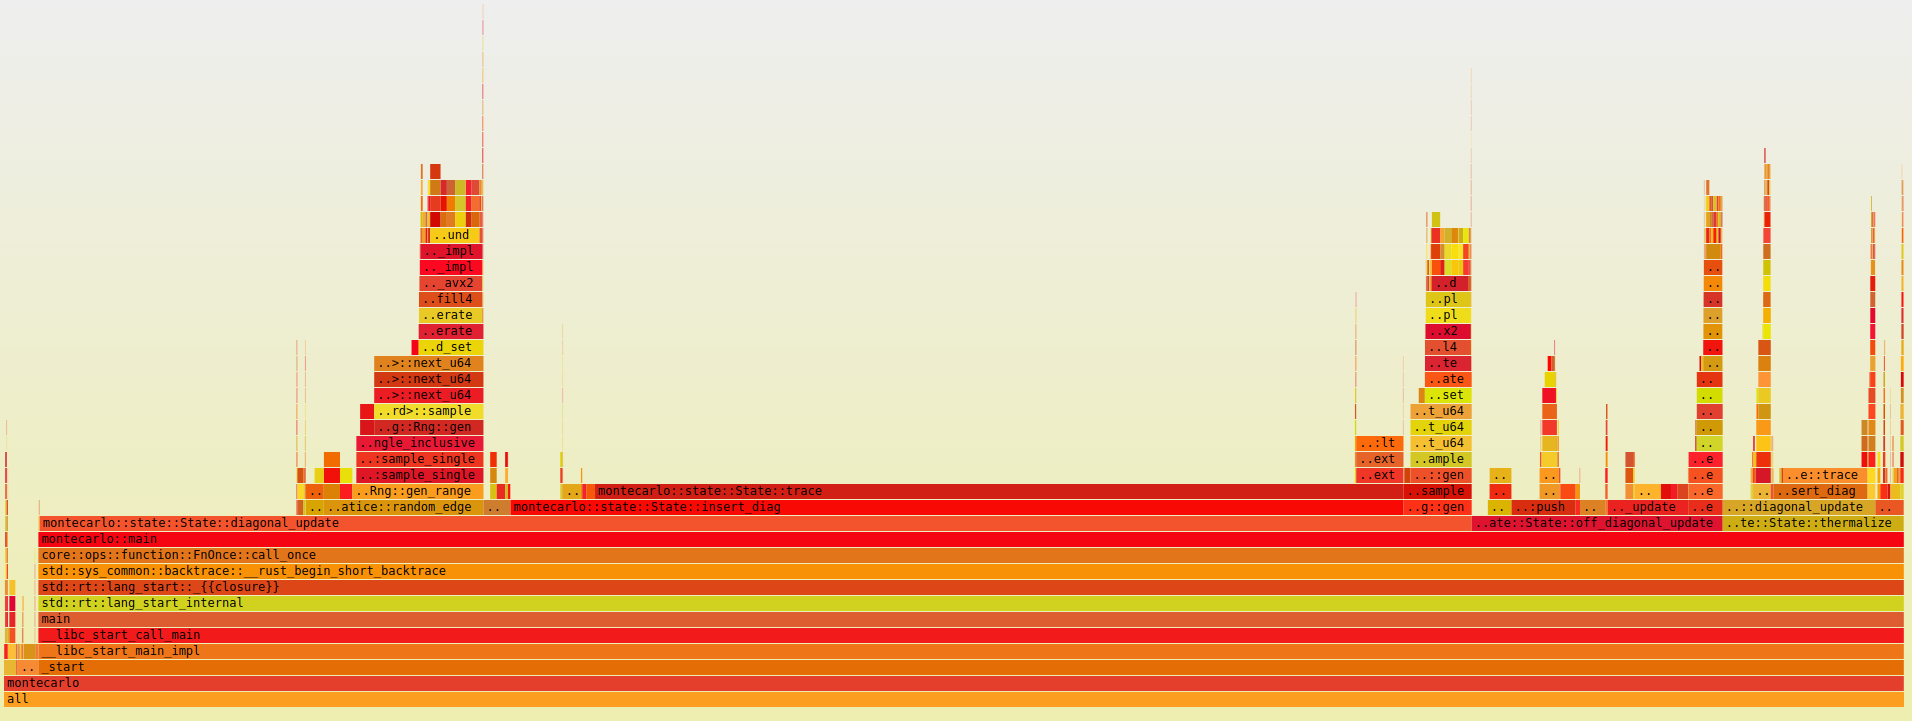
\includegraphics[width=1.0\textwidth]{old_flamegraph.png}
        \caption{A flame graph of the first version of the code. The x-axis represents the proportion of time spent in a function, and the y-axis is the call stack. The wide middle stack is the trace function}
        \label{fig:flame}
    \end{figure}
\subsection*{Algorithm}
The rest of the algorithm is just a standard implementation QMC as seen in the lecture. The only spot that changes is the acceptance probability of adding or removing an operator. The $\bra{\alpha}H_\text{new}\ket{\alpha}$ term for the simple Heisenberg model would always be either 0 or $\nicefrac{1}{2}$ but since we have two bond types we need to include a $J_t$ as well.
\section*{Results}
\subsection*{Question 8}
The first exercise was to plot the expansion order and the operator chain length as a function of Monte Carlo steps. The results of this can be seen in fig \ref{fig:expansion}.
\begin{figure}[H]
        \centering
        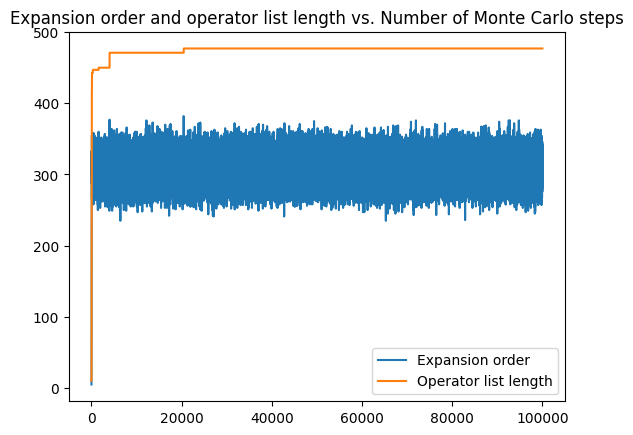
\includegraphics[width=1.0\textwidth]{expansion.png}
        \caption{Expansion order and number of operators on a 4x4 Lattice with $\beta=16$ and $J_1=1.0$}
        \label{fig:expansion}
    \end{figure}    
As expected, the Operator list quickly saturates, while the expansion order fluctuates around a constant value.
\subsection*{Question 9}
The second exercise was to plot the energy for different values of $\beta$ and compare it to exact diagonalization. Since the energy is an affine function of expansion order I didn't repeat the same plot and instead used $J_1$ as the x-axis.
This and all subsequent plots use the bootstrap method to determine error bars. The results of this can be seen in fig \ref{fig:energy}
\begin{figure}[H]
        \centering
        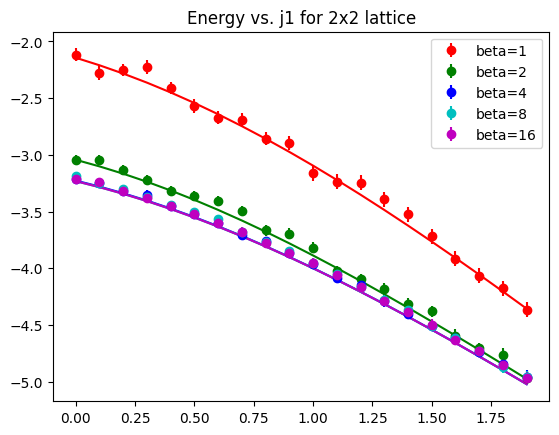
\includegraphics[width=1.0\textwidth]{energy.png}
        \caption{A plot of energy vs $J_1$ for a 2x2 Lattice at different values of $\beta$. The exact diagonalization is drawn as a line, and the Monte Carlo calculations are given as dots with error bars.}
        \label{fig:energy}
    \end{figure}
We see that the energy quickly converges as $beta$ gets larger. We can also see that the algorithm is more stable for higher $\beta$, since the error bars are smaller. But all of them closely follow the expected results.
\subsection*{Question 10}
The last exercise was to plot the staggered magnetization for different system sizes. I again compared this to exact diagonalization for 2x2 but the larger Ls were not possible to calculate exactly. The results can be seen in \ref{fig:magentization}
\begin{figure}[H]
        \centering
        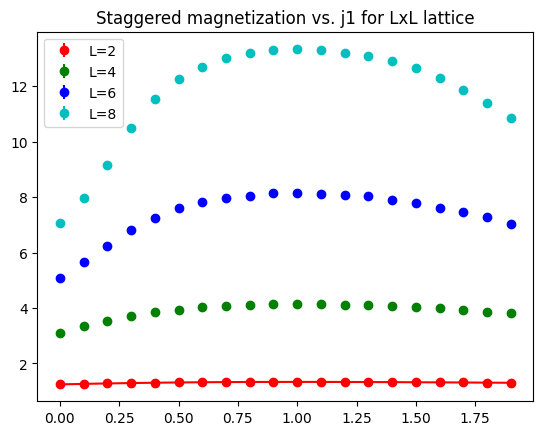
\includegraphics[width=0.45\textwidth]{magnetization.png}
        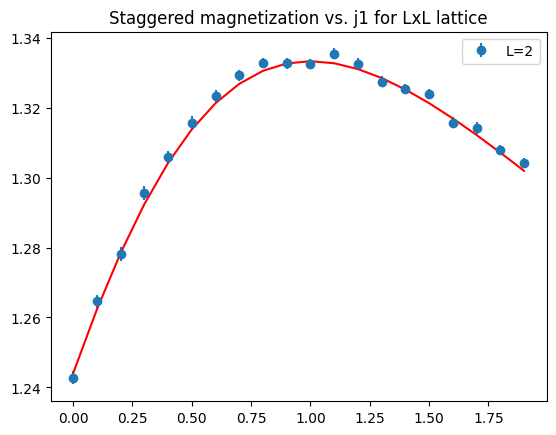
\includegraphics[width=0.45\textwidth]{zoomed_magnetization.png}
        \caption{The staggered magnetization as a function of $J_1$ for different system sizes. $\beta$ was taken to be $8L$ to ensure convergence. The right plot is just a zoomed-in version of $L=2$}
        \label{fig:magnetization}
    \end{figure}
We see in the zoomed version that our results closely follow the exact diagonalization results.
\section*{Bonus question}
Lastly, we will discuss the possibility of adjusting this algorithm to operate on the momentum basis. To make discussion easier, we will look at the one-dimensional Heisenberg model, as the math is simpler there. Recall from the lecture that the Momentum basis was given by
\begin{align*}
    \ket{\text{Rep}(\alpha),m}=k\sum_{k=1}^L e^{\text{i}mk}T^k\ket{\text{Rep}(\alpha)}
\end{align*}
To use this basis we need to split out $H$ into sub-operators such that the no-branching condition is met. We see that each state consists of a sum of rotated versions of the same computational basis state. As such we need to include all rotated versions of a two-site operator if we were to include one. This would map this state onto a superposition, where each possible flip on the representative is performed. Since an operator is fully defined by its action on a basis, we can just split this operator over this superposition and get a new set of operators, each of which represents flipping one of the possible bits of the representative (plus the diagonal part).

The question now becomes how to represent this state. The most obvious solution is to just store the representative of alpha as a bit string (plus the integer m but for now we will restrict ourselves to the m=0 case). This however makes updates hard since flipping two bits requires you to recheck if the vector is still the rep of its family. One solution to this is just to allow all the rotated version of $\alpha$ to appear and treat them as identical states. In the same way, there are different ways to represent the same operator strings by adding identities. However, we see that now we are just flipping bits on alpha and have in a very roundabout way reconstructed the original algorithm.
\section*{Conclusion}
Overall this was a really fun project despite me not figuring out the bonus question. I ended up spending a lot of time optimizing the Markov chain and am quite proud of the performance I managed to achieve. I plan to work on this a bit more in my free time, as I have a few more ideas on how to improve this library and I enjoy this type of coding.
\subsection*{Future work}
\begin{itemize}
  \item There are still some easy low-level optimizations to do regarding avoiding CPU branching in the linking stage
  \item The flame graphs reveal that around 40\% of the time is currently spent generating random numbers. I could look into cheaper pseudo-random generators or try to use the numbers more efficiently (see next point)
  \item One idea of how to get faster convergence is to only propose insertions that have non-zero matrix elements. While this is more expensive to compute, it may lead to higher acceptance rates, lowering the correlation time and improving convergence.
  \item Although Markov chains are an inherently very sequential algorithm, they are cheap enough that running multiple independent chains in parallel should allow for vastly increased sample numbers. Or even with different $J_1$ or $\beta$ values. I would like to play with multithreading on the CPU or maybe even implement QMC in CUDA.
  \item Although the naive approach to momentum basis didn't yield anything, there are a few more possibilities to try out. A different splitting of the operators might yield a better algorithm, as well as coming up with a new way to represent the state in memory. the DFT of $\alpha$ comes to mind.
\end{itemize}

\end{document}
